\documentclass[a4paper,12pt]{report}%define a classe do documento, um artigo.
\usepackage{indentfirst}
\usepackage[ Listing]{algorithm}	
\usepackage{algorithmic}		
%\usepackage{multirow}
\usepackage{dsfont}
\usepackage{graphicx,indentfirst,amsmath,amsfonts,amssymb,amsthm,newlfont}
\usepackage{rotating}
\usepackage{morefloats}
\usepackage{lscape}
\usepackage{amsmath}
\usepackage{listings}
%config link colors
\usepackage{hyperref}
\usepackage{multirow}
\hypersetup{
				colorlinks=true,
				bookmarks=false,
				pdfnewwindow=true,             
				linkcolor=blue,          
				citecolor=blue,        
				filecolor=blue,      
				urlcolor=blue
			}
\usepackage{amsfonts}
\usepackage{amsmath,amssymb}
\usepackage{graphicx}
\usepackage{subfigure}
%\usepackage[latin1]{inputenc}            
%\usepackage[brazil]{varioref}             
%\usepackage[brazilian,portuguese]{babel}
\usepackage{setspace}			

\usepackage[Rejne]{fncychap}			
			
\title{Panca Game Maker -- DOC}

\author{Diogo Fernando Trevisan}

\date{}

\begin{document}

	\begin{titlepage}
		\maketitle
	\end{titlepage}
	
	
	\section{eqs}
	
	$\frac{\partial E(n)}{\partial W_{kj}(n)}$
	
	\chapter{Tileset}\label{tileset}
	\section{Introduction}
		The tileset is a set of \emph{Tiles}. Each Tileset is built using an image. This image is divided into a set of subimages, each of this subimage is a \emph{Tile}. All Tiles in a tileset are square and have the same size (pixels).
	
	
	\section{Tile}
		Each tile of a Tileset as attributes one image (java.awt.Image) and informations about wich directions the player and enemies can pass in this tile, as shows Figure \ref{fig:tile}.
		
	\begin{figure}[h]
		\centering
		
\includegraphics[]{img/tile.png}
		\caption{Tile: a tile have information about wich directions the player can pass. In this example the player can't pass from up to down.}
		\label{fig:tile}
	\end{figure}

	\section{Tileset}
		A tileset is a set of tiles. An image is loaded and a tile size is set. The image of Tileset is cut into as many as possible Tiles. This set of tiles are used to create an Scenary. Figure \ref{fig:tileset} shows an tileset example.
		\begin{figure}[h]
			\centering
			\subfigure[][]{
\includegraphics[width=5cm]{img/tile_input.png}}
			\qquad
			\subfigure[][]{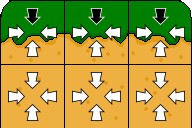
\includegraphics[width=5cm]{img/tile_processed.png}}
			
			\caption{Tileset: the image (a) is cut into various subimages. Each subimage is a \emph{Tile} and have its own attributes.}
		\label{fig:tileset}
	\end{figure}
		
	\section{File Format}
		The tileset can be saved to a file. It is written in binary format, and the format is shown in Listing \ref{listing-tilesetFormat}.
		
		\begin{algorithm}[H]
			\caption{Tileset File Format.}
	      \label{listing-tilesetFormat}
	      \begin{algorithmic}
			\STATE $[int]Number\_tiles\_Y$
			\STATE $[int]Number\_tiles\_X$
			\STATE $[int]Tile\_size$
			
			\FOR{$i=0 \dots Number\_tiles\_Y$}
				\FOR{$j=0 \dots Number\_tiles\_X$}
					\STATE $[int]tile[i][j].terrain\_type$
					\STATE $[bool]tile[i][j].pass\_from\_up$
					\STATE $[bool]tile[i][j].pass\_from\_down$
					\STATE $[bool]tile[i][j].pass\_from\_left$
					\STATE $[bool]tile[i][j].pass\_from\_right$
					\STATE $[int]tile[i][j].image\_height$
					\STATE $[int]tile[i][j].image\_width$
					\FOR{$x=0 \dots tile[i][j].image\_width$}
						\FOR{$y=0 \dots tile[i][j].image\_height$}
							\STATE $[int]tile[i][j].image[x][y]$
						\ENDFOR
					\ENDFOR
				\ENDFOR
			\ENDFOR
		  \end{algorithmic}
		 \end{algorithm}
	\chapter{Graphics}

\section{Sprite}
	Each Sprite consists of an image. The sprite have a display time (in seconds, double), and one collision box with scenary. If none collision box is provided, the entire sprite is a collision box as shows Figure \ref{spriteCollisionBox}.
	
	Each sprite may have a set of collision boxes where is vulnerable and a set of collision boxes where is attacking.
	
	\begin{figure}[H]
		\centering
		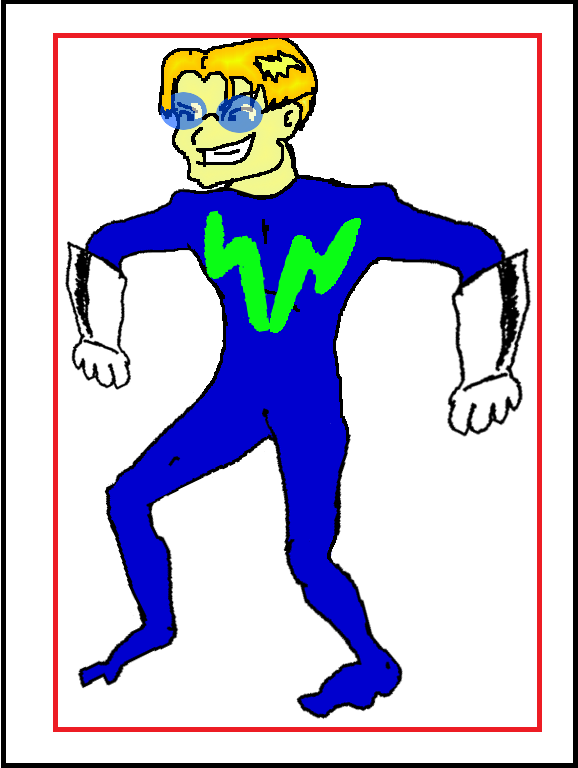
\includegraphics[width=0.45 \textwidth] {img/colisionbox.png}
		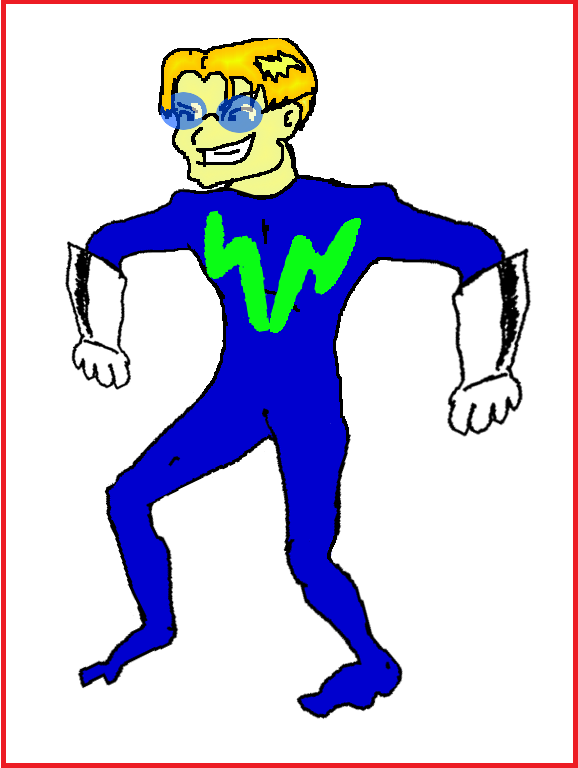
\includegraphics[width=0.45 \textwidth] {img/nocolisionbox.png}
		\caption {Sprite with an collision box (left, in red), and without defining an collision box (right, red).}
		\label{spriteCollisionBox}
	\end{figure}

	\subsection{Drawing the Sprite}
	All Sprite are drawin from the bottom of the point (MIDDLE, 0). The position of the character marks it position and the character is drawn based in this position as shows Figure \ref{fig:spriteDraw}.
	
	\begin{figure}[H]
		\centering
		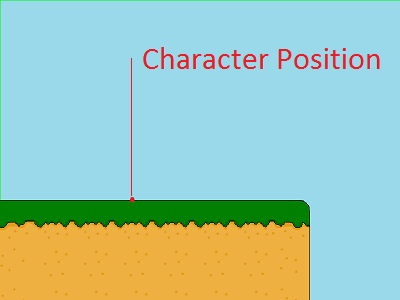
\includegraphics[width=0.32 \textwidth] {img/spritedraw0.png}
		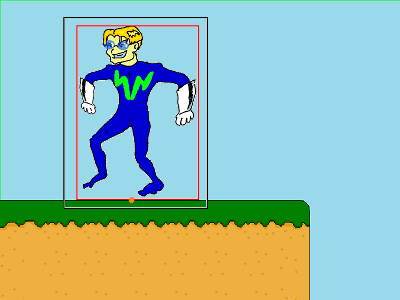
\includegraphics[width=0.32 \textwidth] {img/spritedraw1.png}
		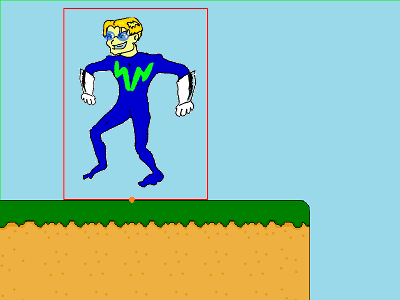
\includegraphics[width=0.32 \textwidth] {img/spritedraw2.png}
		\caption {Positioning the sprite in the character position.}
		\label{fig:spriteDraw}
	\end{figure}
	
	Thus, we can see that it is recommended to always make all sprite animation centering the sprites, and make all character and enemies sprites with the same size.
	
	\subsection{Sprite Coordinate System}
	The Sprite coordinate system is inverse to the bitmaps coordinate system. The (0,0) point is the lower left corner and the (W,H) point is the upper right point as shows Figure \ref{}.
	
	\section{Window \& Drawing}
	The game can support multiple resolutions. Before draw the game to the computer screen it is drawn to a buffer. 
	\textbf{ALL GRAPHIC DATA MUST BE CREATED USING THE INTERNAL RESOLUTION}. Table \ref{} shows the recommended size of graphics and the size of internal window. All data is drawn to the buffer and the buffer is resized in order to fill the screen as can be seen in Figure \ref{fig:display}.
	
	\section{Rendering}
	The Interface \emph{render.Renderable} is used in the \emph{render.Render} class. This Interface  has one method \emph{render(Graphics2D g)} wich takes one argument. This argument is the draw buffer in the size of the internal window. All objects that will be rendered must implement this method. In the GameManager these objects must be put in the render queue -- the Render access the \emph{render} method of all objects in depth order. The usuar order to draw is  Background, Scenary, character (playabe and enemies) and items, and, at last the Head Up Display (HUD).
	
	
	\chapter{Background}
	\section{Introduction}
	
	\section{Background Layer}
		Each background is composed of several layers. Each layer has it's own properties. There are some types of background layers:
		\begin{itemize}
		\item \textbf{ColorBackgroundLayer: } A simple layer that fills the screen with a solid color;
		\item \textbf{ImageBackGroundLayer: } A layer that fills the screen with a image. The image can be stretched to fill the screen or can be tiled horizontally, vertically or in both directions.
		\end{itemize}
		
	\section{File Format}
	
	\chapter{Scenary}

	\section{Introduction}
		Each Scenary is built using a \emph{Tileset}. A Scenary have a number $Y$ of vertical cells and a number $X$ of horizontal cells. Each cell is a reference (pointer) to an \emph{Tile} of the Scenary \emph{Tileset}.
	\section{The Scenary}
		A Scenary is a matrix of Tiles (see \ref{tileset}) called cells. The cells starts from 0 -- height, and 0 -- width. The first cell is upper left corner, as shows fig \ref{fig:scenary}. Each \emph{Scenary} has a tileset, a \emph{Background} and  a visualisation window of $x$ by $y$ pixels wich moves across the scenary and try to center the character. 
		
		\begin{figure}[H]
			\centering
			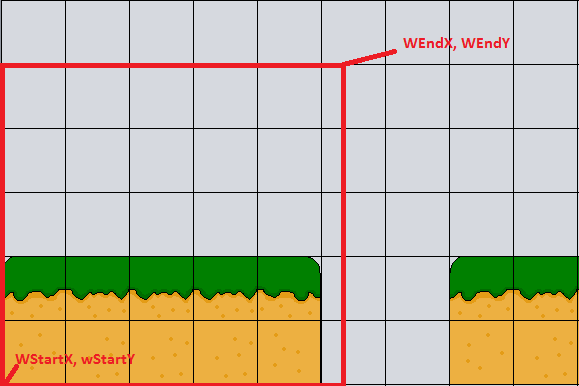
\includegraphics[width=\textwidth]{img/scenary.png}
			\caption{The scenary have a ``moving window'' next to character.}
			\label{fig:scenary}
		\end{figure}
		
		In  game, all scenaries have the same tile size and the same window size. The window is computed using the internal size. If an scenary have $10 \times 200$ tiles and each tile have $32$ pixels, the scenary size will be $320 \times 6400$ pixels, thus, the window size should consider this dimensions. Each window will be resized to fit the \emph{screen resolution} as show Figure \ref{fig:display}.
		
		\begin{figure}[H]
			\centering
			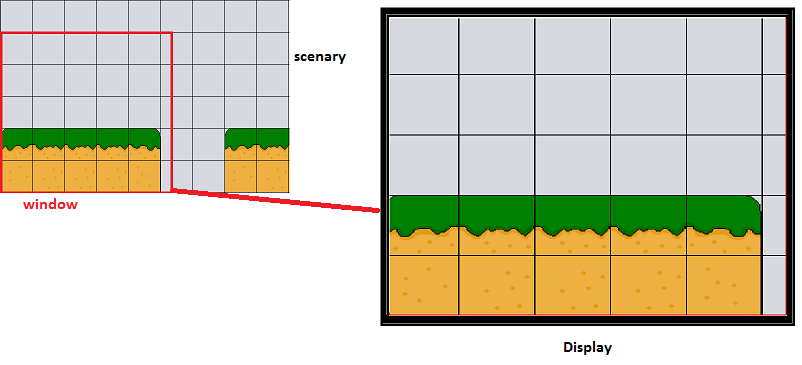
\includegraphics[width=\textwidth]{img/display.png}
			\caption{The buffer is resized to fill up the screen.}
			\label{fig:display}
		\end{figure}
	
		And the scenary coordinate system starts with (X,Y) -- at left bottom, and ends with (X,Y) -- at right upper, as shows Figure \ref{}.
		
		\begin{figure}[H]
			\centering
			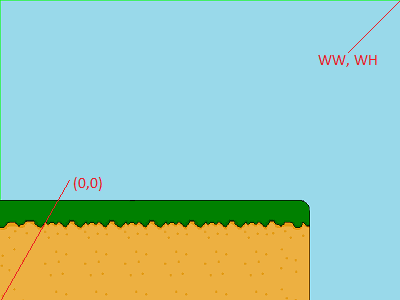
\includegraphics[]{img/scenarycoordinates.png}
			\caption{}
			\label{fig:scenarycoordinates}
		\end{figure}
		
	\section{File Format}
	
	\begin{algorithm}[H]
	\caption{Scenary File Format.}
	  \label{listing-scenaryFormat}
	  \begin{algorithmic}
		\STATE $SAVE\_TILESET()$
		\STATE $SAVE\_BACKGROUND()$
		\STATE $[int]internal\_window\_height$
		\STATE $[int]internal\_window\_width$
		\STATE $[double]gravity$
		\STATE $[int]tile\_number\_y$
		\STATE $[int]tile\_number\_x$
		
		
		\FOR{$i=0 \dots Number\_tiles\_Y$}
			\FOR{$i=0 \dots Number\_tiles\_X$}
				\STATE $a \gets 2$
			\ENDFOR
		\ENDFOR
	  \end{algorithmic}
	 \end{algorithm}
	
	\chapter{ScenaryCollidibleObject}
	Is the most important class. It defines collisions with the scenary, with another objects, enemies etc.
	
	\section{Major Subclasses}
		\begin{itemize}
			\item \textbf{PlayableCharacter} A class to define implementations of the game character.
			\item \textbf{Enemy} A class to define implementations of the enemies.
			\item \textbf{Item} A class to implement items used in the game.
		\end{itemize}
		
	
	\section{Properties}
	\textbf{boolean attack:} check this object attack boxes? If this object can attack others, this must be true.
	
	\textbf{boolean receiveAttak:} This object can receive attacks? if yes, this must be true.
	
	\textbf{boolean checkScenaryCollisionBoxes:} This object collides with another scenary Collision Boxes?
	
	\textbf{boolean multipleCollisions:}
	
	\textbf{int facingSide:} Wich side is this objetct looking?
	
	\textbf{boolean render:} Must be rendered? default=true;
	
	\textbf{boolean onFloor:} Is this object touching the floor?
	
	\textbf{boolean onCeil:} Is this object colliding some tile above it?
	
	\textbf{Vector2D position:} The position in the scenary (not screen);
	
	\textbf{Action actualAction: } The actual object action;
	
	\textbf{Scenary scenaryReference:} The scenary this object is;
	
	
	\chapter{GameItem}

The class GameItem describes several items in the game. 
	\chapter{Action}
	\section{Introduction}
		The action class represents one movement that the character performs when one event happens. The player constrols the character by keyboard, mouse, etc. and a keyboard hit ou a mouse move can be caracterized as an event.
		
		One action have spritesets, wich are activated in the \emph{update()} method. The method updates the action state, character position and etc.
		
		%Each Action can have some restrictions to be activated: some conditions may be satistfies before activate such as some other actions must be activated or deactivates see \ref{creatingAction}.
		
		Each character implementation have a number of actions.
		
		Only one Action can be active. 	
		
		Each Action have a set of Spritesets. Each Spriteset have a name used to select it. It is stored in the \textbf{protected HashMap$<$String, Spriteset$>$ spriteset} attribute.
		
		Each Action have necessry keys, that referencies one Joypad Button.
		
		Te activationkey is the key that activate the action: for example, the SPACE key makes the character jump; if the player press LEFT\_ARROW or RIGHT\_ARROW during the jump then the character will continue jumping but will move left. So, the SPACE is the principal key, called ACTIVATION\_KEY.
		
		
		Each subclass of Ation must implement the methods \textit{update, canActivate \& canDeactivate}.
		
		
	\section{File Format}
	  The action file is saved with its name. For example, to save the action ``SIMPLE\_WALK", the file will have be named ``SIMPLE\_WALK.act" and with the following format:
	  \begin{algorithm}[H]
	      \caption{Action File Format.}
	      \label{algoEvalCuda}
	      \begin{algorithmic}
			\STATE [int]$CLASS\_NAME\_SIZE$
			\STATE [byte*] $CLASS\_NAME$
			\STATE [int] $SPRITESET\_NUMBER$
			\FOR{Each Spriteset}
			  \STATE [int]$SPRITESET\_NAME\_LENGHT$
			  \STATE [byte*]$SPRITESET\_NAME$
			  \STATE [int]$NUMBER\_OF\_LEFT\_SPRITES$
			  \FOR{Each Left Sprite}
				  \STATE [image] $Write\_Image()$						
			      \STATE [double]$DISPLAY\_TIME$			      
				  \STATE [double] $ScenaryCollisionBox\_LowerLeftPoint\_x$
				  \STATE [double] $ScenaryCollisionBox\_LowerLeftPoint\_y$
				  \STATE [double] $ScenaryCollisionBox\_UpperRightPoint\_x$
				  \STATE [double] $ScenaryCollisionBox\_UpperRightPoint\_y$	
				  \STATE [int] $NUMBER\_OF\_ATTACK\_BOXES$
				  \FOR{Each ATK\_BOX}
					\STATE [double] $ATK\_BOX\_LowerLeftPoint\_x$
					\STATE [double] $ATK\_BOX\_LowerLeftPoint\_y$
					\STATE [double] $ATK\_BOX\_UpperRightPoint\_x$
					\STATE [double] $ATK\_BOX\_UpperRightPoint\_y$	
				  \ENDFOR
				  \STATE [int] $NUMBER\_OF\_VULNERABLE\_BOXES$
				  \FOR{Each ATK\_BOX}
					\STATE [double] $VULNERABLE\_BOX\_LowerLeftPoint\_x$
					\STATE [double] $VULNERABLE\_BOX\_LowerLeftPoint\_y$
					\STATE [double] $VULNERABLE\_BOX\_UpperRightPoint\_x$
					\STATE [double] $VULNERABLE\_BOX\_UpperRightPoint\_y$	
				  \ENDFOR
				  
			  \ENDFOR
			  \STATE [int]$NUMBER\_OF\_RIGHT\_SPRITES$
			  \STATE ***SAME AS LEFT SPRITES***
			  % \FOR{Each Sprite}
				  % \STATE [image] $Write\_Image()$
			      % \STATE [double]$DISPLAY\_TIME$			      
				  % \STATE [double] $ScenaryCollisionBox\_LowerLeftPoint\_x$
				  % \STATE [double] $ScenaryCollisionBox\_LowerLeftPoint\_y$
				  % \STATE [double] $ScenaryCollisionBox\_UpperRightPoint\_x$
				  % \STATE [double] $ScenaryCollisionBox\_UpperRightPoint\_y$
				  % \FOR{Each ATK\_BOX}
					% \STATE [double] $ATK\_BOX\_LowerLeftPoint\_x$
					% \STATE [double] $ATK\_BOX\_LowerLeftPoint\_y$
					% \STATE [double] $ATK\_BOX\_UpperRightPoint\_x$
					% \STATE [double] $ATK\_BOX\_UpperRightPoint\_y$	
				  % \ENDFOR
				  % \STATE [int] $NUMBER\_OF\_VULNERABLE\_BOXES$
				  % \FOR{Each ATK\_BOX}
					% \STATE [double] $VULNERABLE\_BOX\_LowerLeftPoint\_x$
					% \STATE [double] $VULNERABLE\_BOX\_LowerLeftPoint\_y$
					% \STATE [double] $VULNERABLE\_BOX\_UpperRightPoint\_x$
					% \STATE [double] $VULNERABLE\_BOX\_UpperRightPoint\_y$	
				  % \ENDFOR
			  % \ENDFOR
			\ENDFOR
		  \end{algorithmic}
		 \end{algorithm}
		 
		 
		 
	\section{Class Members}
	
	This section show the necessary attributes in the class Action. These attributes are allocated in superclass Action but must be set in the subclasses.
	
	\paragraph{String[] necessarySpritesets:} The name of the necessary spritesets to this action can be used. Use the ``addSpriteset'' to add spritesets.
	\paragraph{String[] spritesetsDescriptions:} The descriotion of the necessary spritesets.
	\paragraph{Hashtable$<$String, Boolean$>$ toActivateRestrictions: } The restrictions to activate this action. A hashtable containing ``AnotherActionName, status(actve/inactive)''.
	\paragraph{ Hashtable$<$String, Boolean$>$ toDeactivateRestrictions: } The restrictions to deactivate this Action.
	\paragraph{String name: } The name of this Action.
	\paragraph{boolean canDeactivate():} Return true if can deactivate, else return false. 
	\paragraph{boolean canActivate(): } Return true if can activate the action.
	\paragraph{Vector<String> necessaryButtons: } the button names that the action needs. This buttons must exist in the Joypad class.
	\paragraph{void update(double timeElapsed): }  the most important method. Receives as parameter the elapsed time since the last update. Can use the joypad to verifies if some important key where pressed.
	\paragraph{Vector<String> activationButtonsNames:} The name of the buttons that can activate the Action.
	
	
	
	\section{Creating Your Own Action}
	Each Action have a different behavior. Each one can have it's own attributes. But all must:
	
	\begin{itemize}
	\item {update it's behaviour} For example, for a jump, the action will make the character position increase or decrease. The action have acces to the joypad and its states and the key buffer. If its jumping and the player press LEFT the char will move left.
	\item{Clear the Input } making a call to \emph{cleanInput()}.
	\end{itemize}
	
	The initialization \textbf{must}:
	\begin{itemize}
	\item {Initialize \emph{necessarySpritesets}:} This is a String array and each position contains the name of a \emph{spriteset} that must be created and set. Its used in the visual editor and used to verifie if the action is valid.
	\item{initialize \emph{spritesetsDescriptions}:} This is a String array containing the description of the necessary spritesets.
	\item{Set the Action's \emph{name}:} The name is essential, so, it must be initialized.
	\item{Initialize \emph{activationButtonsNames}:} It is an array with the name of all buttons that can activate the Action. It is a String array with the Button names defined in \emph{Joypad}. If the action need buttons to initialize (for example the action that runs when no key is pressed) the \emph{activationButtonsNames = null}.
	\item{Initialize \emph{necessaryButtons}:} It is an array of Strings, each position have the name of one Joypad button. Again, if the Action don't need an key the \emph{necessaryButtons = null}.
	\end{itemize}
	\chapter{Joypad}
	\section{Introduction}
		The Joypad class acts just like an joypad. It have some buton variables thar can be active or inactive. The character used this states to update.
		
		All buttons have public access to simplify.
		
		When a key is typed, the event handler (java.awt.event.KeyListener) verifies the key and store the status in ``Hashtable$<$Integer, Integer$>$ buttonStates''. If the state is BUTTON\_TYPED the action \textbf{must} set it to BUTTON\_OFF in it's update method. Just use the ``Action.cleanInput'' method in the ``Action.update'' after doing the update.
		
		
		The Joypad.buttonBuffer is a buffer with buttons in the order that are pressed (or  threated).
	\section{Buttons}
		The buttons have 3 possible states:
		\begin{itemize}
			\item \textbf{public static final int BUTTON\_OFF = 0}: the button is released.
			\item \textbf{public static final int BUTTON\_TYPED = 1}: the button was typed (pressed one time and released).
			\item \textbf{public static final int BUTTON\_HOLD = 2}: the button was pressed and hold.
		\end{itemize}
		If the button status = \textbf{BUTTON\_TYPED} the character \emph{update} method must set it to \textbf{BUTTON\_OFF} after the use.
		
	\section{Attributes}
	
	\paragraph{Hashtable$<$String, Integer$>$ buttonCodes: } The name of buttons of controller, and the key code associated with it. The Action uses this map to update it state. For example: `` `BUTTON\_UP',67'', will map the button up to the key of asc CODE 67. 
	
	The Joypad can have as many buttons as the user need, but the button names must be accordling to the Action.necessaryButtons. For example, Action x have $necessaryButtons = [``BUTTON\_UP'', ``BUTTON\_X'']$ then the Joypad.buttonCodes must have the key maps for ``BUTTON\_UP'' and ``BUTTON\_X''.
	
	
	
	\section{Joypad Templates}
	Template creates a Joypad with some buttons.
	
	\begin{table}[H]
    \caption{Possible collisions with the scenary.}
    \label{tab:scenaryCollisionTypes}
    \centering
	
    \begin{tabular}{|l|p{5cm}|}
		\hline
		\textbf{Template} 				& \textbf{Buttons} \\
		\hline
		TEMPLATE\_JOYPAD\_10\_BUTTONS 	&  UP,  DOWN, LEFT,  RIGHT,  PAUSE,  A,  B,  C,  D, SPECIAL \\
		\hline
	\end{tabular}
	\end{table}
	
	
	\chapter{Character}

	\section{Introduction}
		Each character extends the Character class. The \emph{update} method must be implemented. 
		
		
		
	Each Character consists of a set of actions.
	
	To create an character, must firstly create actions, then add the actions to character. After this, the method \textbf{String buildCharacter()} must be called in order to check and create character actions dependecy.
	
	Each Action have its dependencies, in other words, to create an Action you need to create all Actions necessary to this Action. All these actions are added to the character.
	
	\section{File Format}
	\begin{algorithm}[H]
	    \caption{Character description File Format.}
	    \label{algoEvalCuda}
	    \begin{algorithmic}
			\STATE CREATE\_DIR
			\STATE [F][STRING] CLASS\_NAME
			\STATE [F][STRING]CHAR\_NAME
			\FOR {EACH ACTION}
				\STATE WRITE\_ACTION\_INSIDE\_DIR
				\STATE [F][STRING]ACTION\_NAME
			\ENDFOR
			%\STATE [F][STRING] NUMBER\_OF\_BUTTON\_MAPS
			%\FOR {EACH BUTTON\_MAP}
			%	\STATE [F][INT] KEY\_CODE
			%	\STATE [F][STRING] ACTION\_NAME
			%\ENDFOR
		\end{algorithmic}
	\end{algorithm}
	
	\section{Collision Types}
	\begin{table}[H]
    \caption{Possible collisions with the scenary.}
    \label{tab:scenaryCollisionTypes}
    \centering
	
    \begin{tabular}{|l|c|}
		\hline
		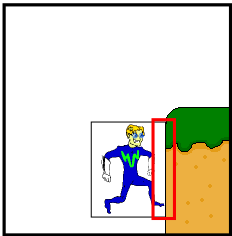
\includegraphics[width = 3cm]{img/leftright_collision.png} & COLLISION\_SCENARY\_LEFT\_RIGHT \\
		\hline
		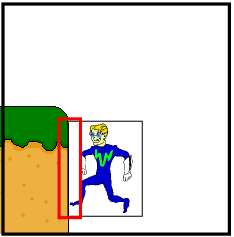
\includegraphics[width = 3cm]{img/rightleft_collision.png} & COLLISION\_SCENARY\_RIGHT\_LEFT \\
		\hline
		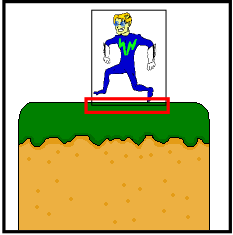
\includegraphics[width = 3cm]{img/updown_collision.png} & COLLISION\_SCENARY\_UP\_DOWN \\
		\hline
		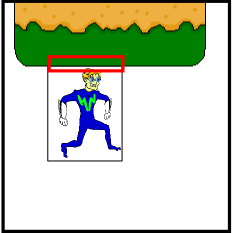
\includegraphics[width = 3cm]{img/downup_collision.png} & COLLISION\_SCENARY\_DOWN\_UP \\
		\hline
		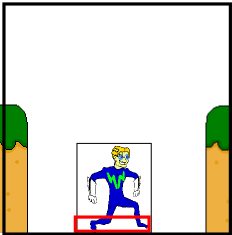
\includegraphics[width = 3cm]{img/outscenary_collision.png} & COLLISION\_SCENARY\_OUT\_SCENARY \\
		\hline
	\end{tabular}
	\end{table}
	
	\section{The Update Method}
	The update method must be implemented in the subclass.  It's the most important method, wich will determine all characters caracterstics.
	
	Fisrtly, analise inputs in the Joypad.buttonBuffer. For each button pressed verifies if can activate the associated action (by the ACTIVATION\_KEY). 
	\chapter{Physics}

	\section{Collision Box}
	Each collision box have four points: upper--left, upper--right, lower--left and lower--right. This points represents the translated points: the points are created accordling to Sprite coordinates, but the collision is computed using the translated points (computed from the Character position). In the Character collision detection the actual Sprite must have its collision boxes translated to the actual Character position.
	\begin{figure}[H]
		\centering
		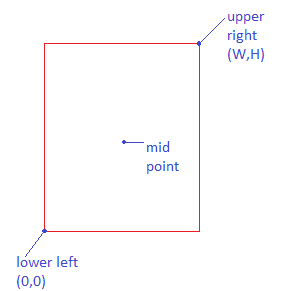
\includegraphics[]{img/collisionboxcoordinates.png}
		\caption{Collision Box coordinates Accordling to the Sprite coordinates. }
		\label{fig:collisionBox}
		
	\end{figure}
	\section{Game Manager}
Is a class to load the configuration 


\section{File Format}
The game file is a text file containing:

	\begin{algorithm}[H]
		\caption{Action File Format.}
		\label{algoEvalCuda}
		\begin{algorithmic}
			\STATE [int] INTERNAL\_WINDOW\_WIDTH
			\STATE [int] INTERNAL\_WINDOW\_HEIGHT
			\STATE [int] SCENARY\_NUMBER
			\STATE [string] CHARACTER\_FILE\_NAME
			\FOR {EACH SCENARY}
				\STATE [string] SCENARY\_NAME
			\ENDFOR
		\end{algorithmic}
	\end{algorithm}
\end{document}